\begin{lstlisting}
理论与实现:
1. 费米子
2. 玻色子
3. mq中如何构造这些算子

支持功能:
1. 运算
  a. 算子间相乘
  b. 加上一个数
2. Transfrom
\end{lstlisting}

We often see operators in the equations of quantum mechanics. Operators and wave functions are the cornerstones of quantum theory. The state of the quantum system is represented by the wave function; Observables are represented by operators. An operator acts on a quantum state as a linear transformation, mapping one quantum state to another.

In MindQuantum, quantum operators is a combination of basic gates, including unitary gates, measurements, and noisy channels. MindQuantum supplies a number of special operators natively, with the opportunity to extend these operators for more advanced use cases, including Fermion operators, Qubit operators, TimeEvolution operators, etc. Table \ref{operators_table} shows an overview of the three operators.

\begin{table}[htbp]
    \centering
    \caption{The overview of operators in MindQuantum}
    \label{operators_table}  %表格名字,用于正文中引用表格
    % \resizebox{\textwidth}{!}{
    \begin{tabular}[htbp]{l|l|l}
        \textbf{Operator}       & \textbf{MindQuantum representation}          & \textbf{Examples}                                                   \\
        \hline
        Qubit operators         & $mindquantum.core.operators.QubitOperator$   & QubitOperator('X0 Y3', 0.5) + 0.6 * QubitOperator('Z1')             \\
        Fermion operators       & $mindquantum.core.operators.FermionOperator$ & FermionOperator('0', 1 + 2j) + FermionOperator('$0^{\wedge}$', 'a') \\
        TimeEvolution operators & $mindquantum.core.operators.TimeEvolution$   & TimeEvolution(QubitOperator('Z0 Y1', 'a'))                          \\
        \hline
    \end{tabular}
    % }
\end{table}


\subsubsection{Common Operators in MindQuantum}
\paragraph{Fermion Operators}
In the microscopic world, many tiny particles are not fixed, but have "spin" characteristics, which can be understood as "the deflection of a magnet in a magnetic field". Spins can be large or small, but their values are quantized, and they can only take integer or half-integer multiples of Planck constant. Particles with different spins are divided into two types. Those with integer values are called bosons. Those with half-integer spin values are called fermions. Common photons are bosons, and electrons are fermions.

In MindQuantum, fermion is represented by the fermion operator wrapped by the $mindquantum.core.operators.FermionOperator$, which are the basic operators to describe a fermionic system, including molecular system, and they follow the anti-commutation relationship.

For example, \verb|FermionOperator('4^ 3 9 3^')| is used to represent the fermion $\alpha_4^\dagger \alpha_3 \alpha_9 \alpha_3^\dagger$. In particular, the zero operator and the identity operator are expressed in forms \verb|FermionOperator()| and \verb|FermionOperator('')|, respectively.

In addition, a $FermionOperator$ object can be parameterized, and its second parameter represents the coefficient of the single fermion operator.

\begin{lstlisting}
from mindquantum.core.operators import FermionOperator
para_op = FermionOperator('0 1^', 'x')
print(para_op)

para_dt = {'x':2}
op = para_op.subs(para_dt)
print(op)
\end{lstlisting}
Output:
\begin{lstlisting}
-x [1^ 0]
-2 [1^ 0]
\end{lstlisting}

\paragraph{Qubit Operators}
$mindquantum.core.operators.QubitOperator$ is the wrapper of Qubit operators. A $QubitOperator$ is an operator acting on multiple qubits and can be represented as: $coefficient * operator_{local}[0] × … × operator_{local}[n-1]$, where $×$ represents the tensor product. An $operator_{local}$ is a Pauli operator ($'I'$, $'X'$, $'Y'$, or $'Z'$) which acts on one qubit.

In mathematical notation a term of $QubitOperator$ can be, for example, $0.5 * ‘X1 X5’$, which means that a Pauli $X$ operator acts on qubit $1$ and qubit $5$, while the identity operator acts on all the other qubits. Terms like this add up to form a Hamiltonian, e.g., $0.5 * ‘X1$ $Y3’ + 0.3 * ‘X0$ $Z2’$, coded as \verb|QubitOperator('X1 Y3', 0.5) + 0.3 * QubitOpera-| \verb|tor('X0 Z2')|.The code below calculates the representing matrix of \verb|0.3 * QubitOperator('X0 Z2')| and shows that a $QubitOperator$ can is equivalent to a superposition of multiple Pauli operators:
\begin{lstlisting}
from numpy import kron
from mindquantum.core.gates import X, Z, I
op = 0.3 * kron(kron(Z.matrix(), I.matrix()), X.matrix())
print(op)
ham = 0.3 * QubitOperator('X0 Z2')
print(ham.matrix())
\end{lstlisting}
Output:
\begin{lstlisting}
[[ 0.   0.3  0.   0.   0.   0.   0.   0. ]
 [ 0.3  0.   0.   0.   0.   0.   0.   0. ]
 [ 0.   0.   0.   0.3  0.   0.   0.   0. ]
 [ 0.   0.   0.3  0.   0.   0.   0.   0. ]
 [ 0.   0.   0.   0.   0.  -0.3  0.   0. ]
 [ 0.   0.   0.   0.  -0.3  0.   0.   0. ]
 [ 0.   0.   0.   0.   0.   0.   0.  -0.3]
 [ 0.   0.   0.   0.   0.   0.  -0.3  0. ]]
  (0, 1)	(0.3+0j)
  (1, 0)	(0.3+0j)
  (2, 3)	(0.3+0j)
  (3, 2)	(0.3+0j)
  (4, 5)	(-0.3+0j)
  (5, 4)	(-0.3+0j)
  (6, 7)	(-0.3+0j)
  (7, 6)	(-0.3+0j)
\end{lstlisting}
Notice that MindQuantum uses big-endian for qubit ordering. The ordering is the opposite of the tensor product structure of the state space. So a 3-qubit quantum register \textbf{qreg} with wave-function $\ket{\psi}=\ket{q_2\otimes q_1 \otimes q_0}=\ket{q_0 q_1 q_2}$  has qreg[0]=$\ket{q_0}$, qreg[1]=$\ket{q_1}$, qreg[2]=$\ket{q_2}$. Therefore, Similarly for representing unitary matrices of a circuit. $U=U_2 \otimes{U_1}\otimes{U_0}=U_2 U_1 U_0$ would have $U_2$ acting on qreg[0], $U_1$ acting on qreg[1] and $U_0$ acting on qreg[2]. In addition, a Hamiltonian composed of QubitOperators should be a hermitian operator, thus requires the coefficients of all terms must be real.

\paragraph{TimeEvolution Operators}
In quantum mechanics, studying only fixed states allows us to have a deeper understanding of the basic principles of quantum mechanics. But in reality, all systems (except the Universe as a whole) interact at least somewhat with other systems, and the state $\ket{\phi}$ of a quantum mechanical system changes with time, so it is of great significance to study the time evolution of such state.

MindQuantum supports the time evolution operator, $mindquantum.core.operators.TimeEvolution$, which will perform the following evolution: $\ket{\phi(t)} = e^{-iHt}\ket{\phi(t_0)}$, describing the evolution of the state of a closed quantum system in continuous time. The Hamiltonian $H$ should be either parametric or non-parametric $QubitOperator$. Besides, if the $QubitOperator$ has multiple terms, a first-order Trotter decomposition will be used. The code below shows how to use the operator $TimeEvolution$ to get the quantum circuit corresponding to a given Hamiltonian (see Fig.~\ref{2.5_TimeEvolution_circuit}):
\begin{lstlisting}
from mindquantum.core.operators import TimeEvolution, QubitOperator
q1 = QubitOperator('Z0 Y1', 'a')
q2 = QubitOperator('X0 Z1', 'b')
ops1 = q1 + q2
ops2 = q2 + q1
TimeEvolution(ops1).circuit.svg()
TimeEvolution(ops2).circuit.svg()
\end{lstlisting}
\begin{figure}[h]
    \centering
    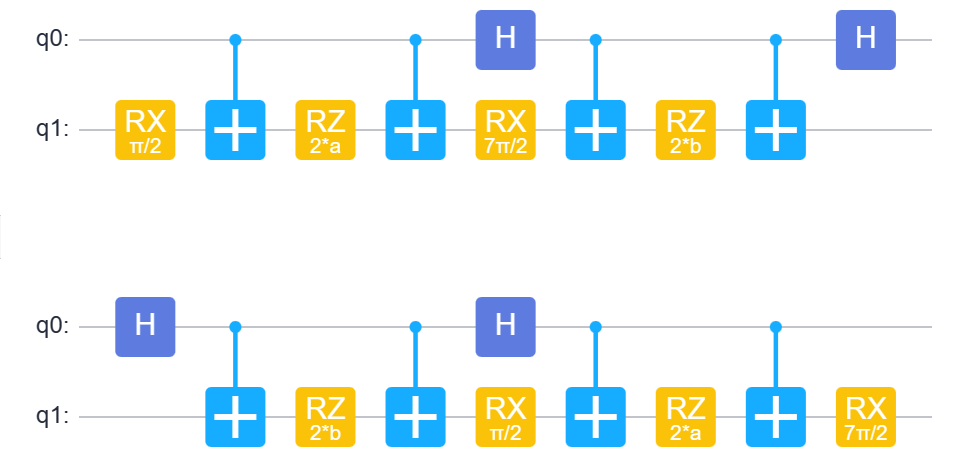
\includegraphics[width=0.7\linewidth]{2.5_figures/2.5_TimeEvolution_circuit.png}
    \caption{quantum circuit obtained by $TimeEvolution$}
    \label{2.5_TimeEvolution_circuit}
\end{figure}


\subsubsection{Operations of MindQuantum Operators}

\paragraph{Basic Operations}
Mindquantum supports some basic arithmetic operations, including:
\begin{itemize}
    \item Multiply by another operator:
          \begin{lstlisting}
from mindquantum.core.operators import QubitOperator
q1 = QubitOperator('X0 Y3', 0.5)
q2 = QubitOperator('X0 Z1', 0.3)
ops1 = q1 * q2
    \end{lstlisting}
    \item Add a number:
          \begin{lstlisting}
from mindquantum.core.operators import QubitOperator
q1 = QubitOperator('X0')
ops1 = q1 + 0.5
print(ops1.matrix())
q2 = QubitOperator('Z0')
ops2 = q2 + 0.5
print(ops2.matrix())
    \end{lstlisting}
          Output:
          \begin{lstlisting}
  (0, 0)	(0.5+0j)
  (0, 1)	(1+0j)
  (1, 0)	(1+0j)
  (1, 1)	(0.5+0j)
  (0, 0)	(1.5+0j)
  (1, 1)	(-0.5+0j)
\end{lstlisting}
\end{itemize}

\paragraph{Other Operator Features}
\begin{itemize}
    \item Most Operators also have a unitary matrix representation, which can be accessed by Operator.$matrix()$.
    \item Most Operators can be converted to a different data type version by using Operator.$astype()$.
    \item
    \item
\end{itemize}

\paragraph{Operator Functions}
Mindquantum also supplies a number of advanced functions for Operators in mindquantum.core.operators libraries. Here are some common ones:
\begin{itemize}
    \item $commutator()$: Calculate the commutator of two operators.
          \begin{lstlisting}
from mindquantum.core.operators import QubitOperator, FermionOperator, commutator
qub_op1 = QubitOperator("X1 Y2")
qub_op2 = QubitOperator("X1 Z2")
commutator(qub_op1, qub_op1)  # 0
commutator(qub_op1, qub_op2)  # (2j) [X2]
    \end{lstlisting}
    \item $count\_qubits()$: Count the number of qubits before deleting unused qubits.
          \begin{lstlisting}
from mindquantum.core.operators import QubitOperator,FermionOperator, count_qubits
qubit_op = QubitOperator("X1 Y2")
count_qubits(qubit_op)  # 3
fer_op = FermionOperator("1^")
count_qubits(fer_op)  # 2
    \end{lstlisting}
    \item $down\_index()$: Return the index order in spin-free orbit of a given spin-down orbital according its index number in spin-down orbitals. We set the default spin-free orbit to even-odd-even-odd (0,1,2,3,...). Spin-down orbitals ($\alpha$ orbitals) have odd indexes and spin-up orbitals have even ones.
          \begin{lstlisting}
from mindquantum.core.operators import down_index
down_index(1)   # 3
    \end{lstlisting}
    \item $up\_index()$: Return the index order in spin-free orbit of a given spin-up orbital according its index number in spin-up orbitals.
          \begin{lstlisting}
from mindquantum.core.operators import up_index
up_index(1)   # 2
    \end{lstlisting}
\end{itemize}
